\documentclass[aspectratio=169]{beamer}
\usepackage[utf8]{inputenc}
\usepackage[T1]{fontenc}
\usepackage{svg}

\setbeamercolor{section in toc}{fg=black}
\setbeamercolor{subsection in toc}{fg=black}

\title{Open Data: \\ Receive it Yourself}
\date[ISPN ’80]{Datenspuren 2022, Dresden}
\author[]{Tassilo, 0xA, Marenz (dump@dvb.solutions)}

\usetheme{dvb}

\AtBeginSection[]{
  \begin{frame}
    \begin{tikzpicture}
      \fill[rounded corners,dvbyellow,rotate around={30:(-1,0.5)}] (-20.5,0) rectangle (-0.5,2);
      \fill[rounded corners,dvbyellow,rotate around={30:(-1,0.5)}] (-20.5,3) rectangle (-0.5,5);
      \node (logo) at (-18,2) {
        \textbf{ \LARGE \textbf{ \myfont \secname } }
      };
  \end{tikzpicture}
  \end{frame}
}

\newcommand*{\myfont}{\fontfamily{pag}\selectfont}

\begin{document}

\begin{frame}\titlepage
\end{frame}
  
\begin{frame} 
 %\includesvg{dvbdump}
\frametitle{Roadmap} 
%\framesubtitle{The proof uses \textit{reductio ad absurdum}.} 

\tableofcontents

\end{frame}

\section{Radio \& VDV 420}

% =================================================

\begin{frame}
\frametitle{Receiving data}
\centering
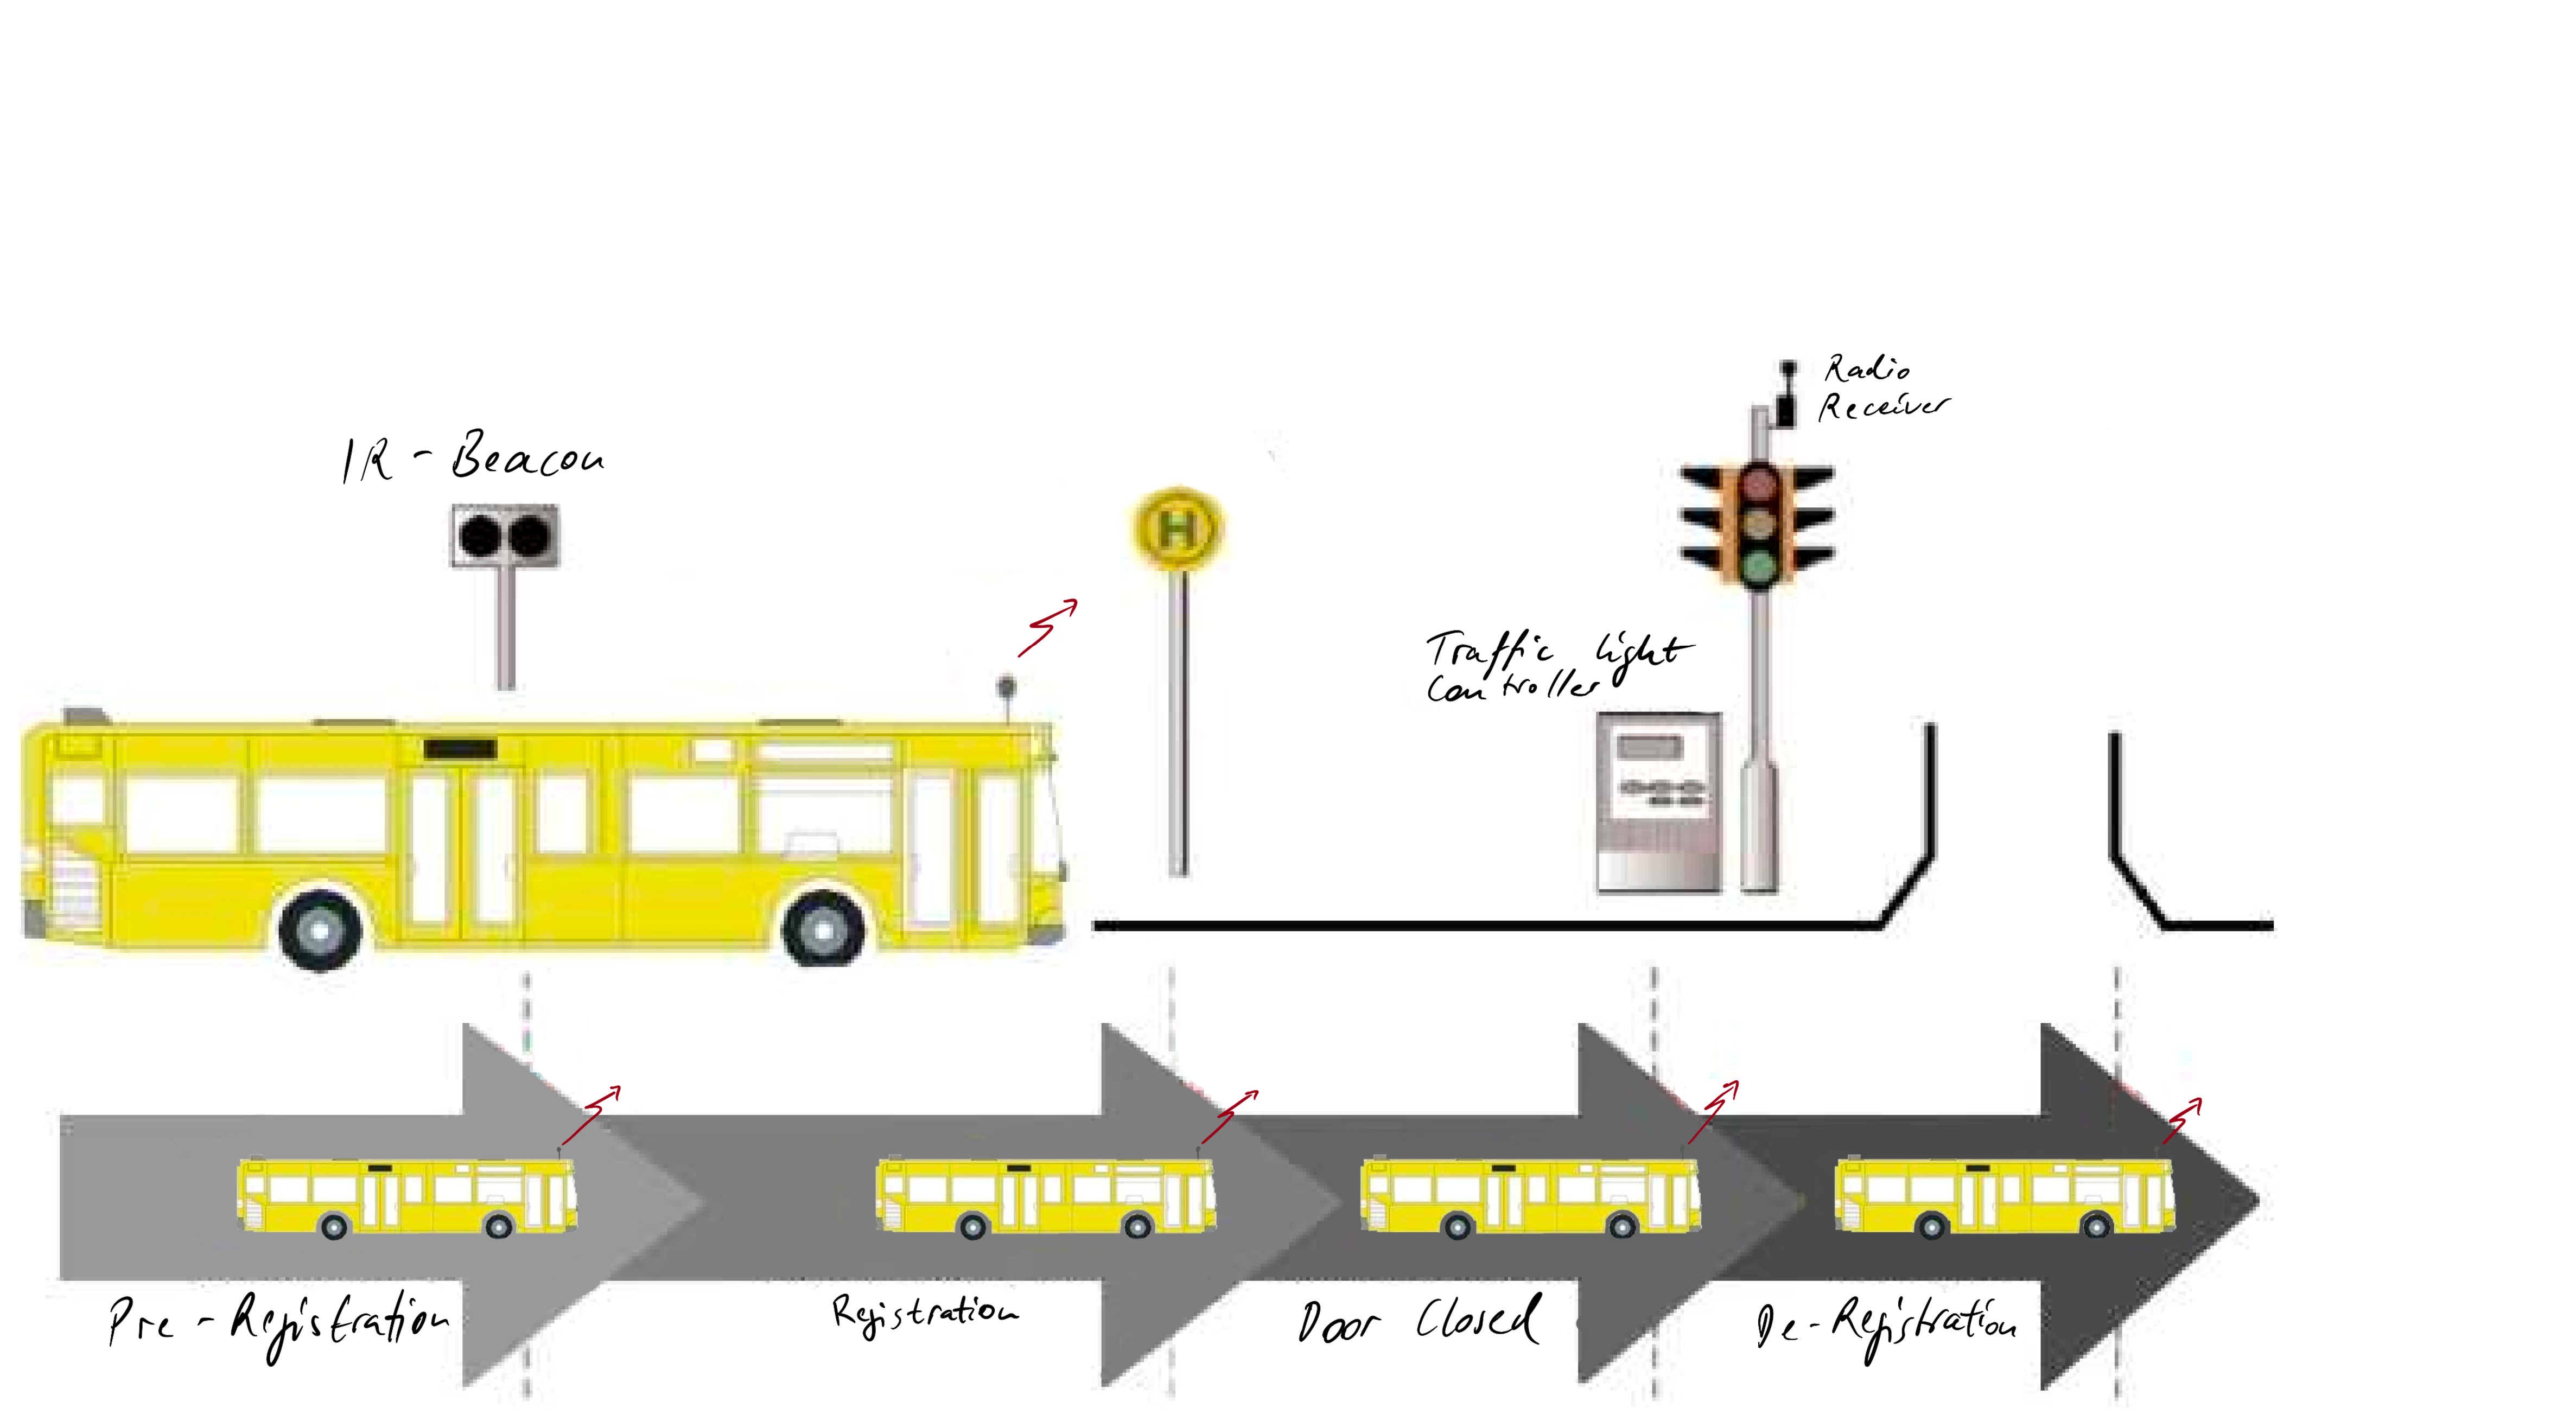
\includegraphics[width=0.8\textwidth]{figs/lsa-beeinflussungs-stecke.pdf}
\end{frame}

% =================================================

\begin{frame}
\frametitle{Receiving data}
\centering
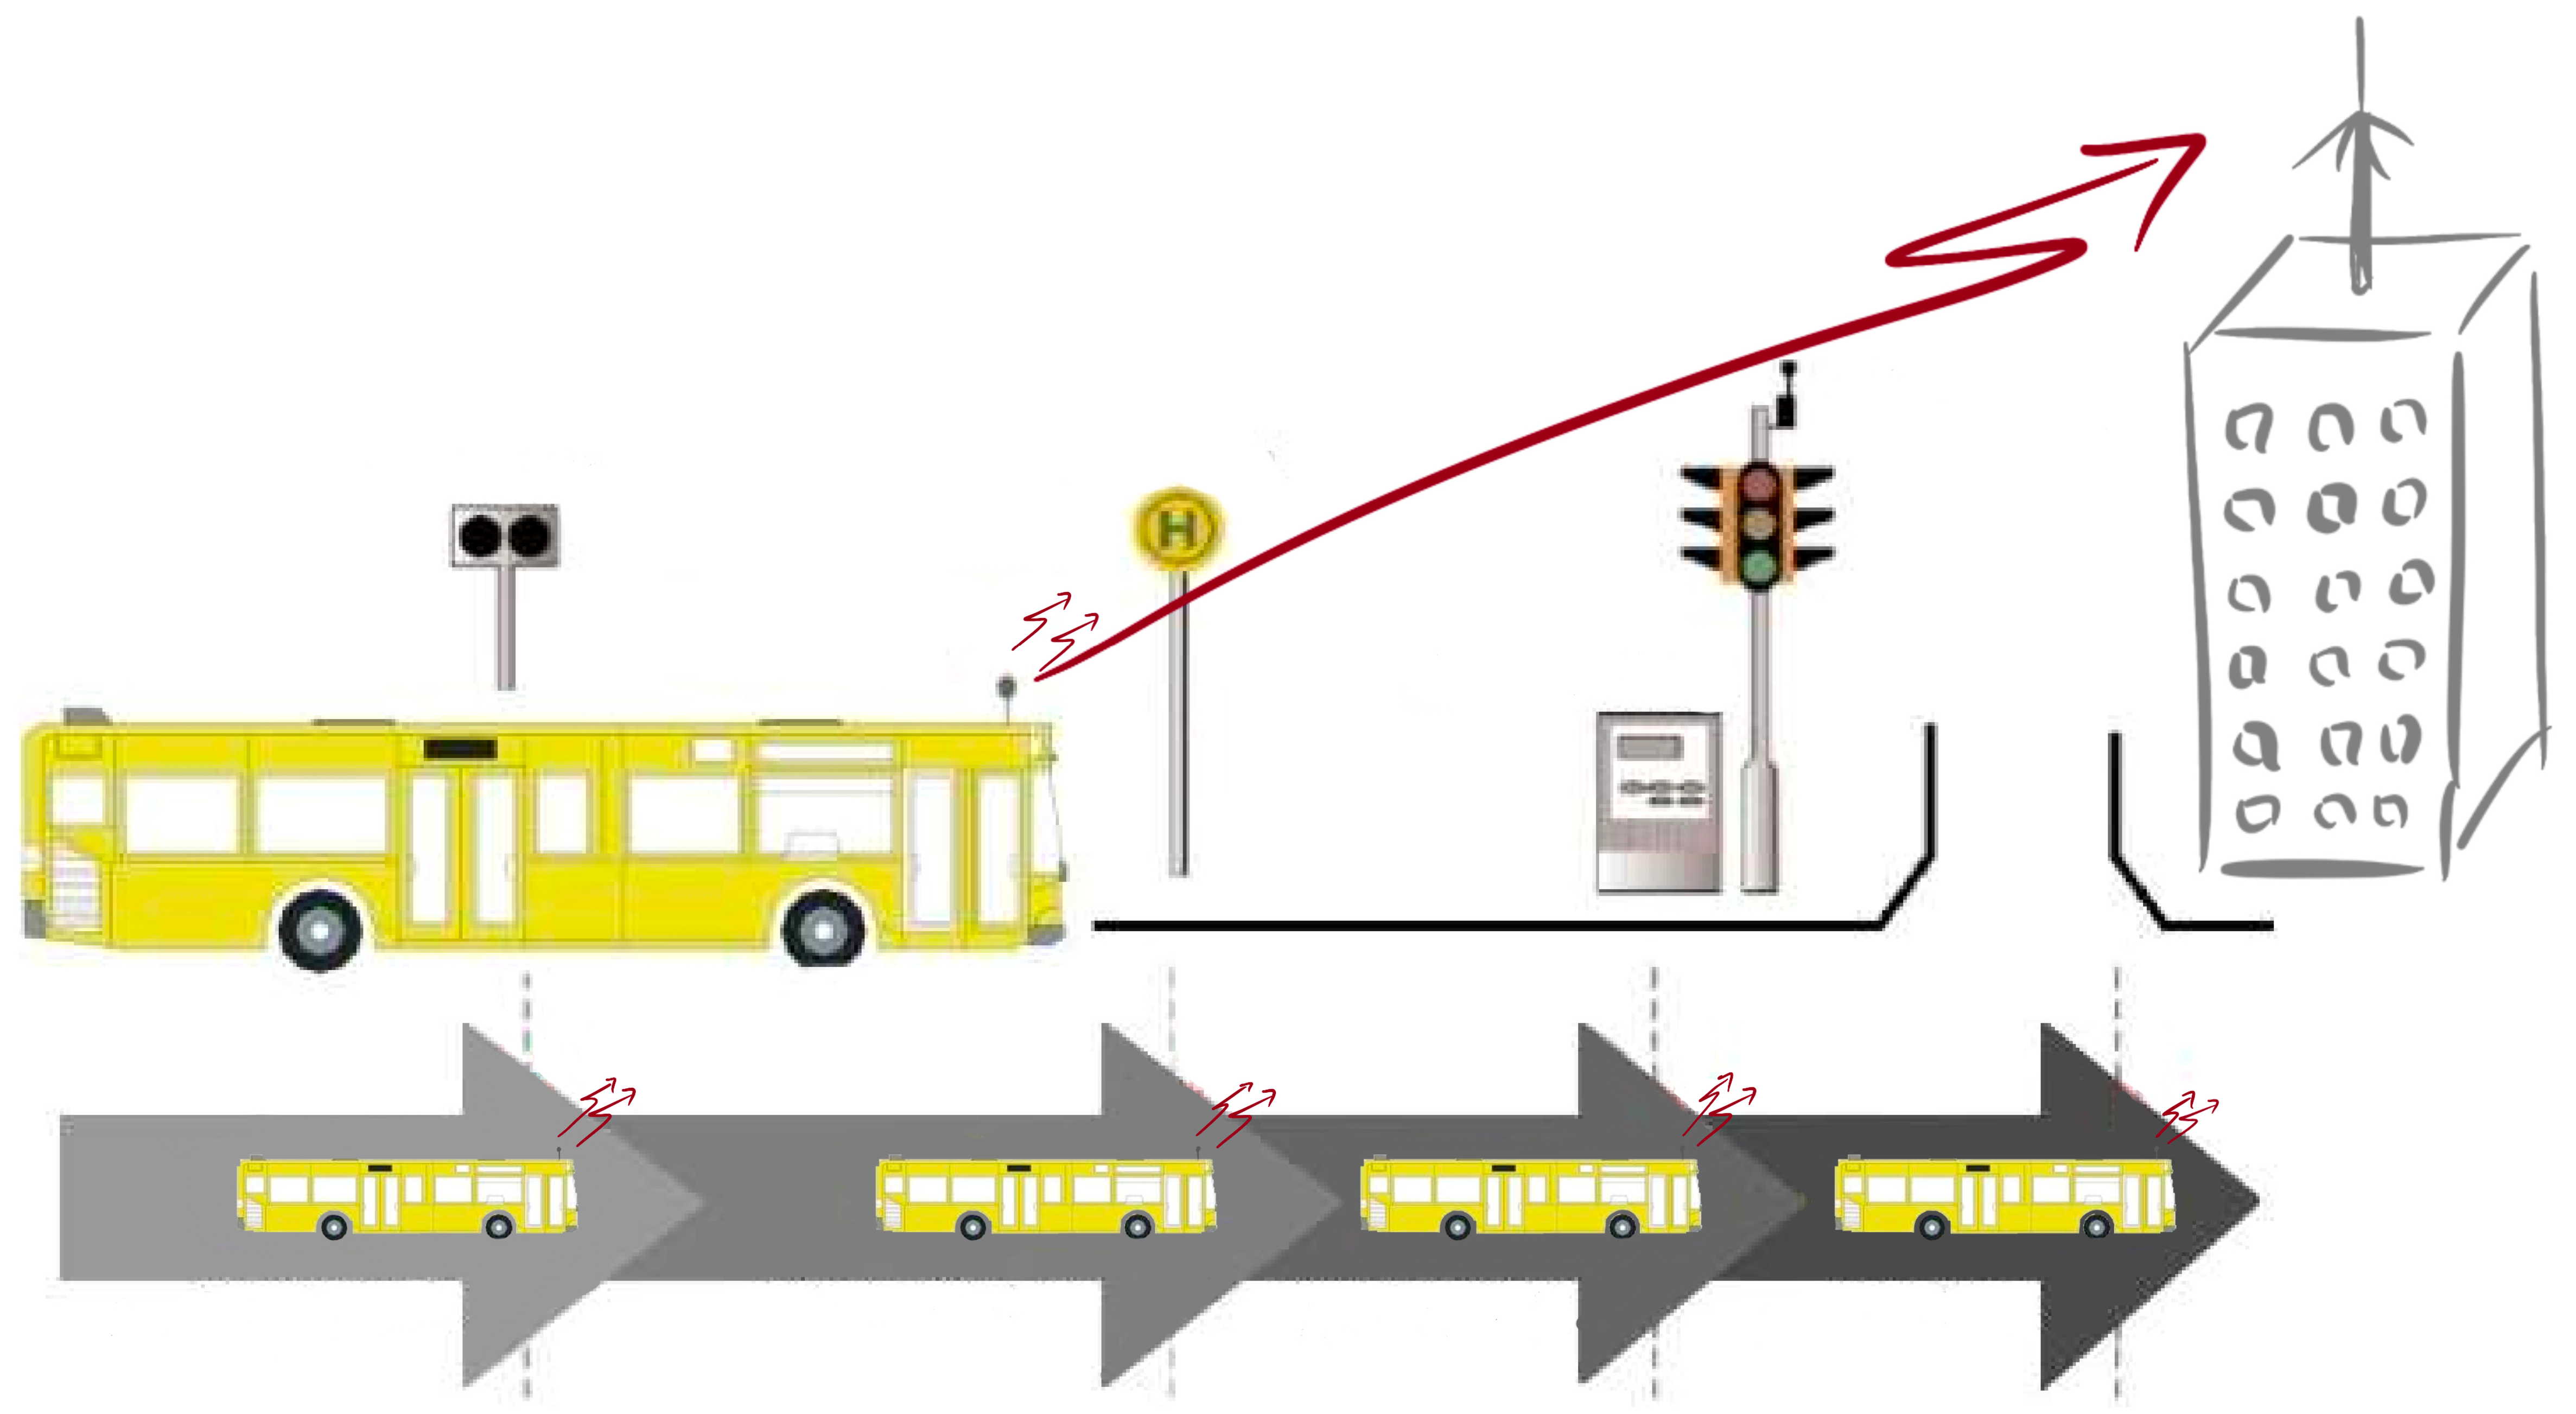
\includegraphics[width=0.8\textwidth]{figs/lsa-beeinflussungs-stecke-mit-antenne.pdf}
\end{frame}

% =================================================

\begin{frame}
\frametitle{Receiving data}
\centering
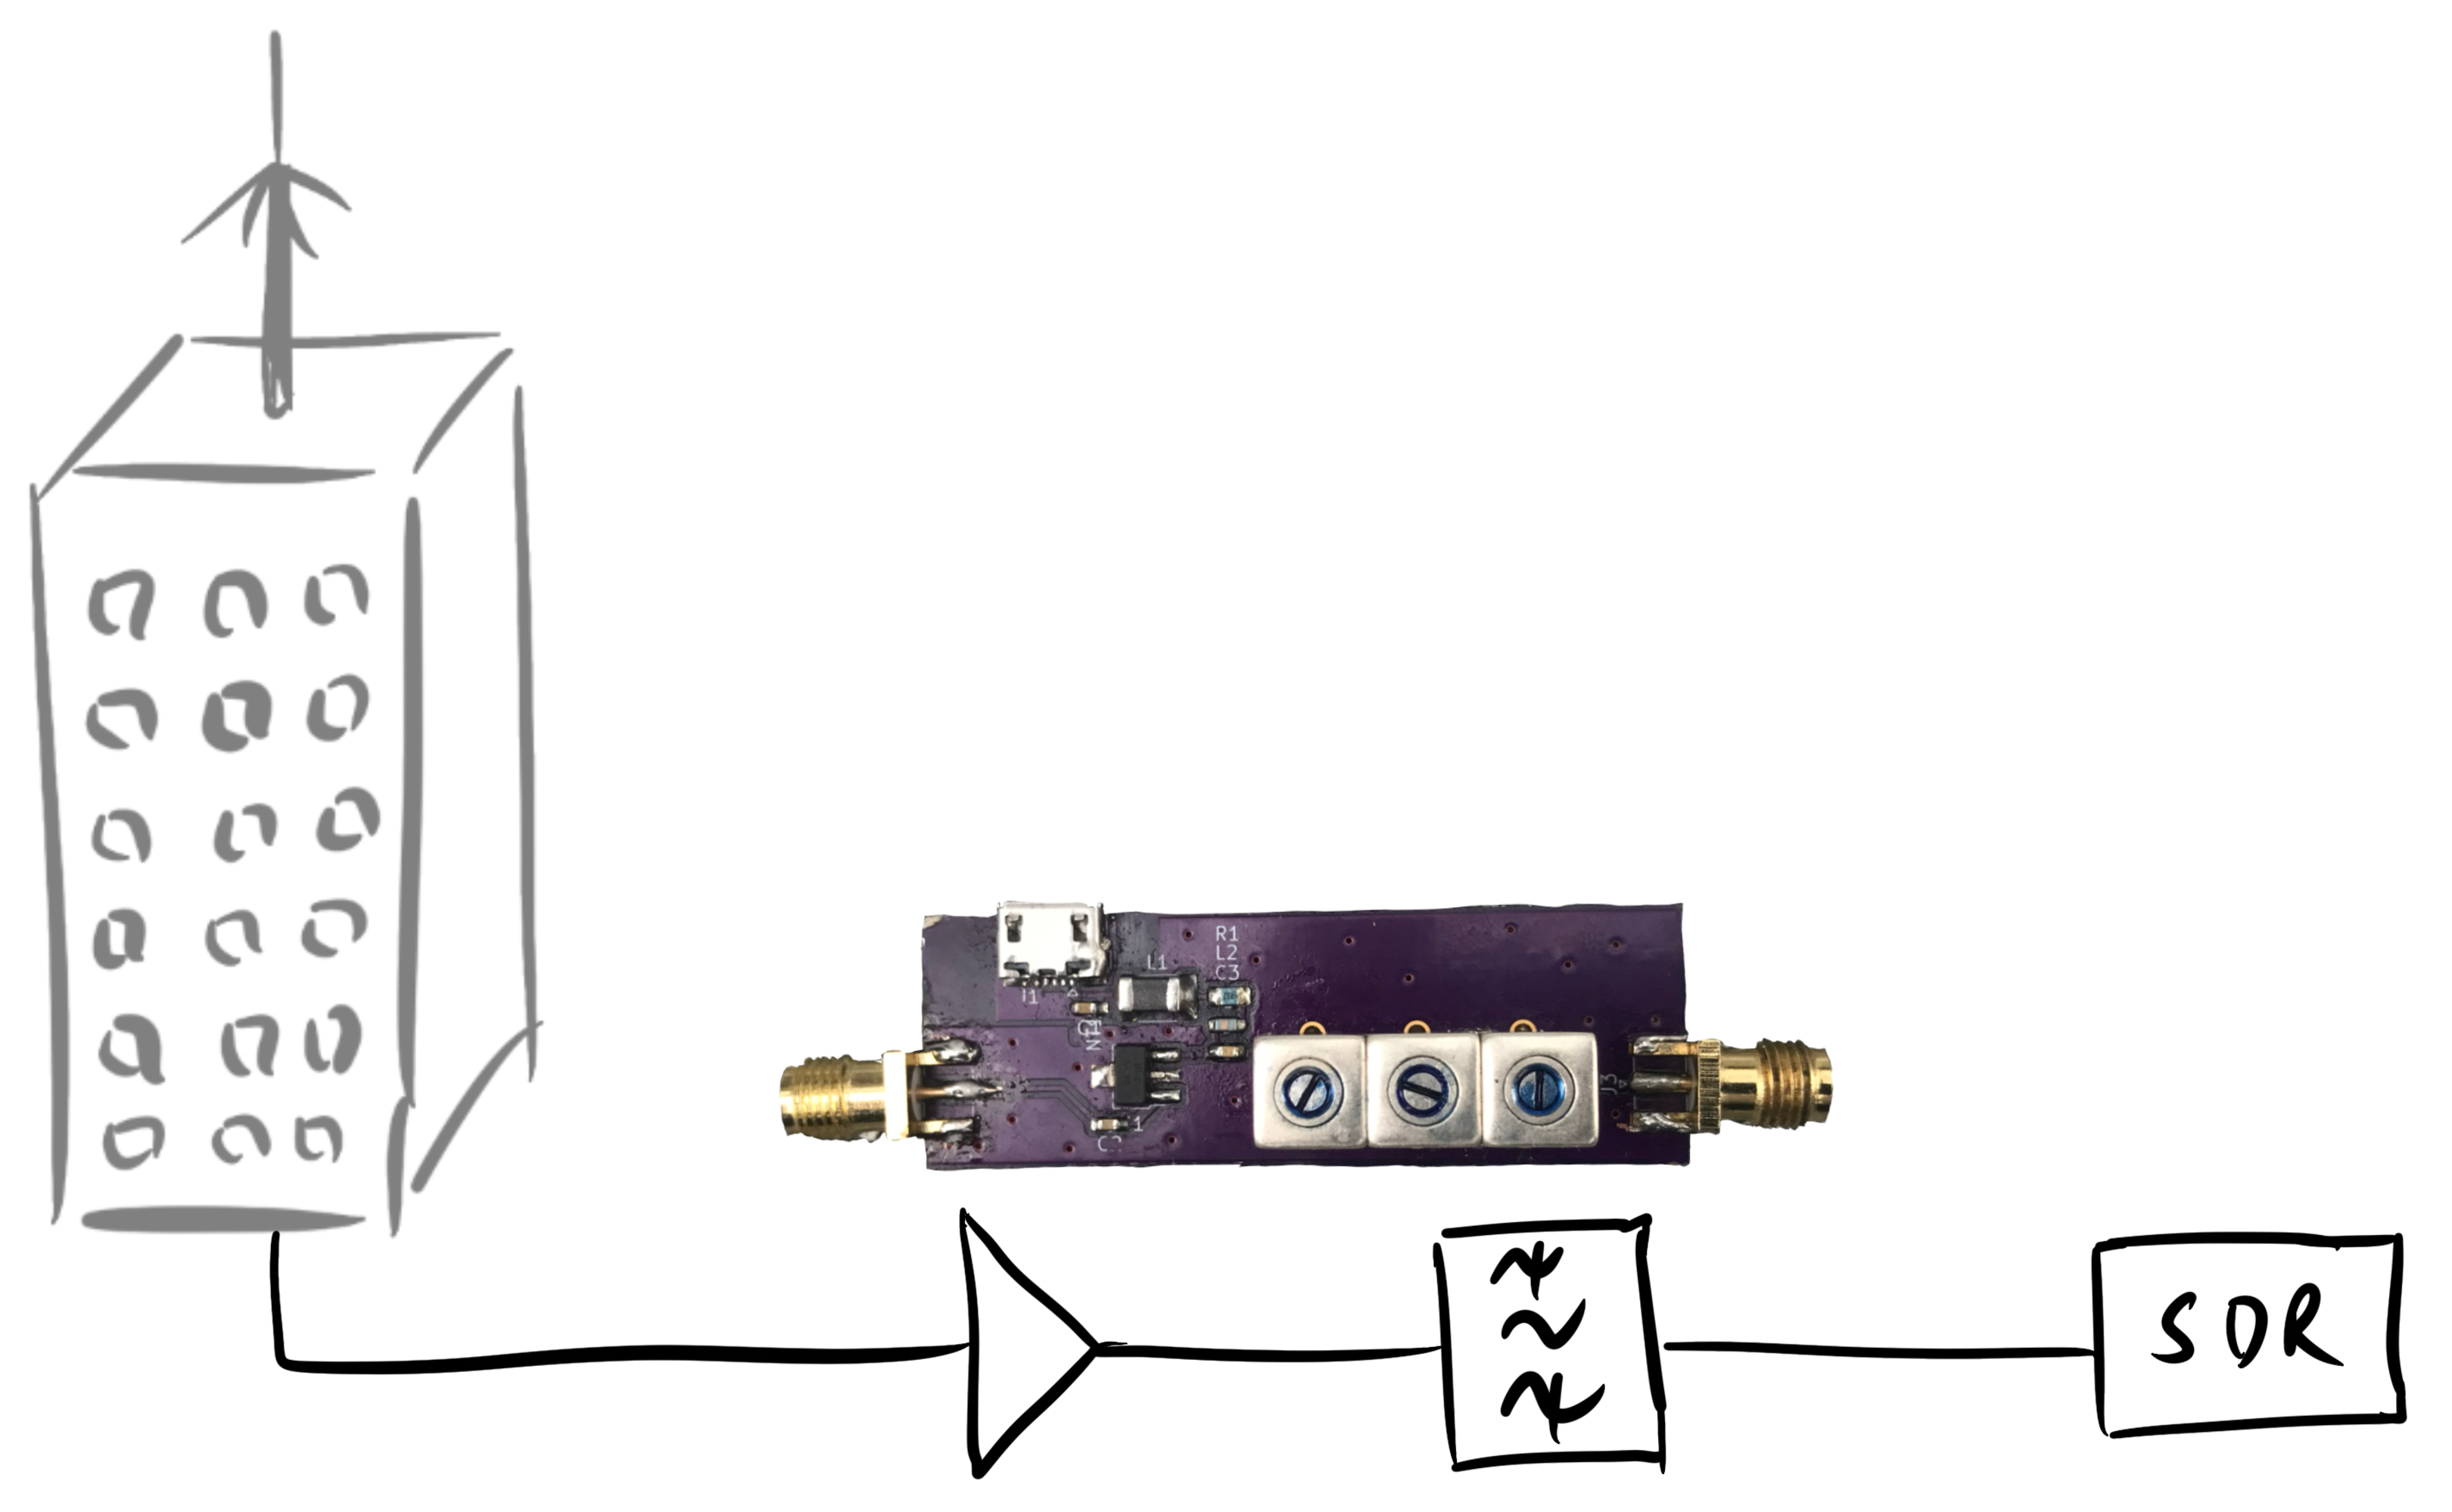
\includegraphics[width=0.7\textwidth]{figs/antenna-filter.pdf}
\end{frame}

% =================================================

\begin{frame}
	\begin{itemize}
		\item R09 telegrams of trams and busses standardized in \href{https://knowhow.vdv.de/documents/420/}{VDV 420}
		\item dresden uses R09.16
		\item what data do we receive?
		\begin{itemize}
			\item Tram identification data: line number, run number, destination number
			\item Location data: traffic light id, direction, registration\_type
			\item and some other
		\end{itemize}
	\end{itemize}
\end{frame}

% =================================================

\begin{frame}
\frametitle{Receiving data}
\begin{figure}
\centering
% https://opus4.hbz-nrw.de/opus45-bast/frontdoor/deliver/index/docId/2595/file/V353+BF+Gesamtversion.pdf
% page 25
\begin{columns}
\column{.5\linewidth}
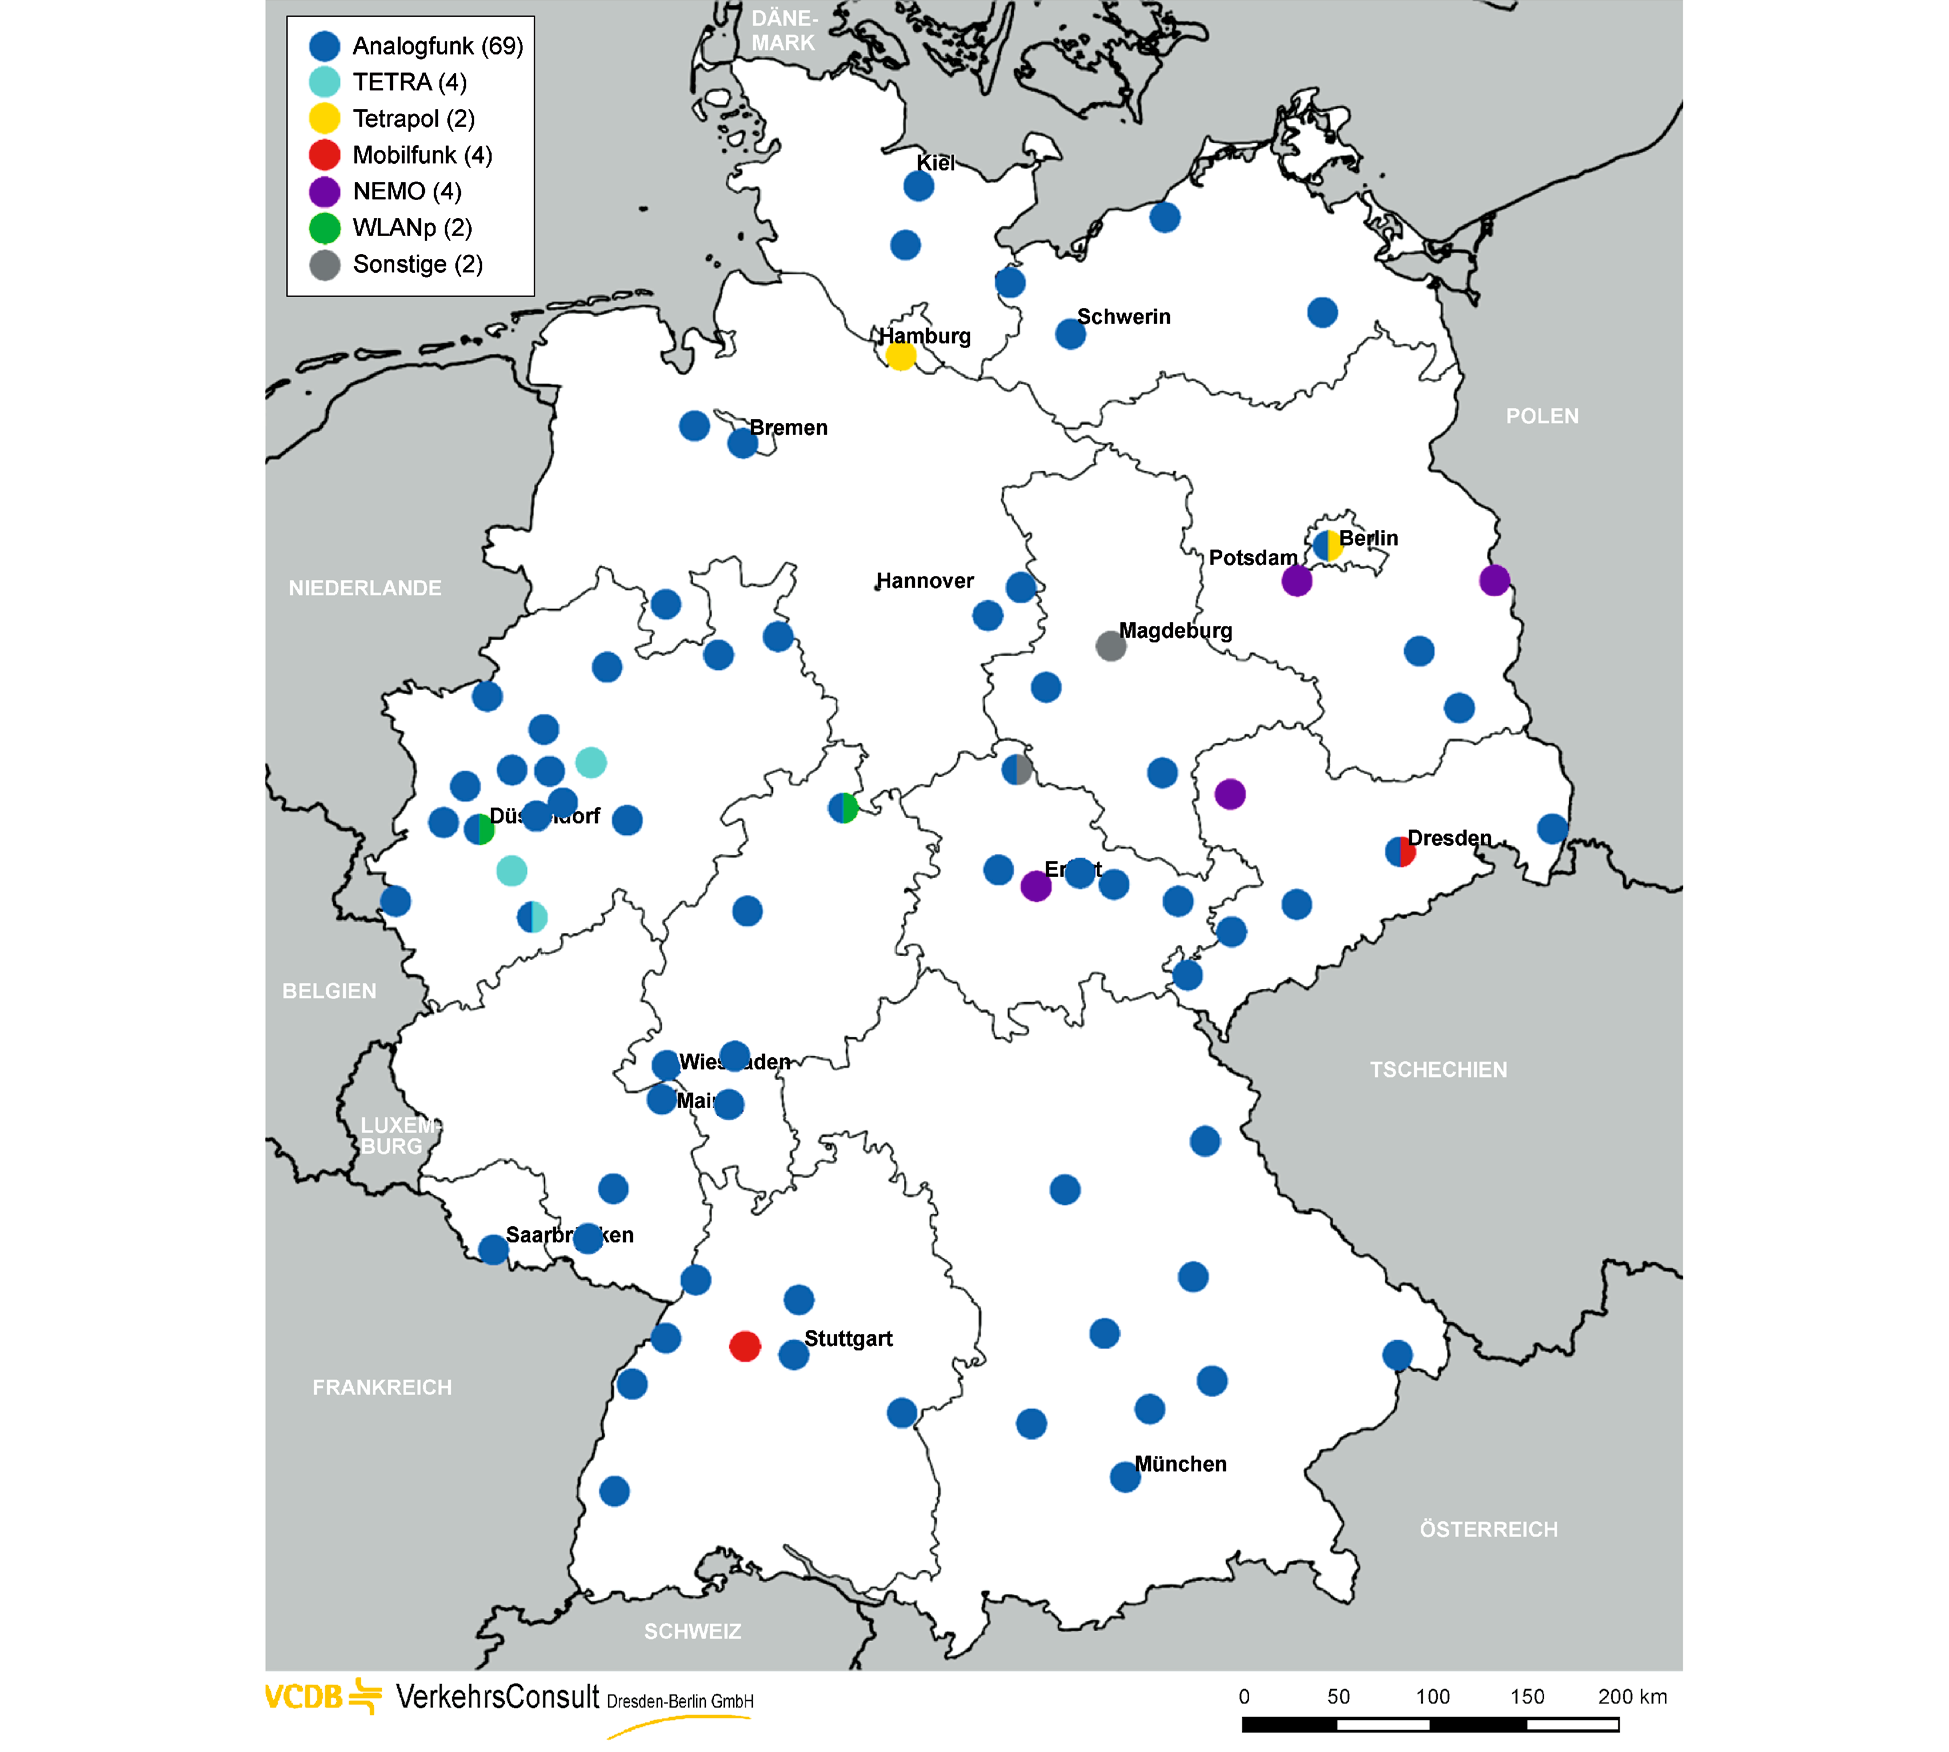
\includegraphics[height=0.8\textheight]{figs/vcdb-map-ampelbeeinflussung.png}
\column{.5\linewidth}
\caption{Map showing some of the locations with traffic lights, controlled by public transport. Blue points use the standard we already implemented.}
\end{columns}
\end{figure}
\end{frame}

% =================================================

\section{Soul Extrating Information \& Mapping }

%TODO: oxa


% =================================================

\section{Architecture \& Infra }

% =================================================

\begin{frame}
\frametitle{What Shit we have currently running}

\begin{figure}

\centering
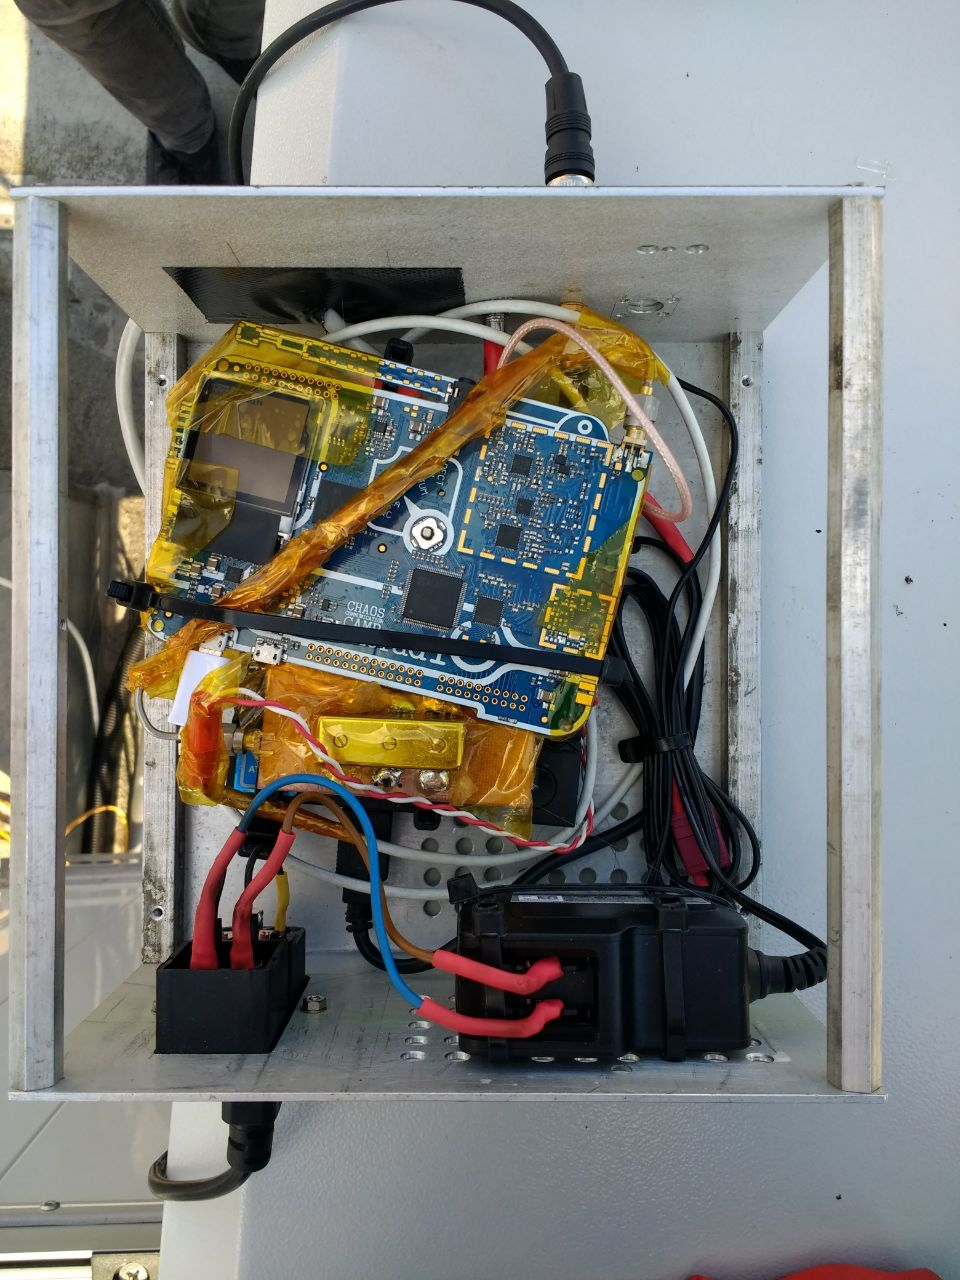
\includegraphics[height=0.94\textheight, angle=90]{figs/station_barkhausen.jpg}
\caption{ Station Barkhausenbau }
\end{figure}

\end{frame}

% =================================================

\begin{frame}
\frametitle{What Shit we have currently running}

\begin{tikzpicture}


\end{tikzpicture}

\end{frame}


\section{Call for Action}

\section{Questions}

\end{document}
